% \documentclass[11pt,a4paper]{article}

\usepackage[english,italian]{babel}
\usepackage[utf8]{inputenc}

\usepackage{hyperref}
\hypersetup{
    bookmarks=true,         % show bookmarks bar?
    % unicode=false,          % non-Latin characters in Acrobat’s bookmarks
    % pdftoolbar=true,        % show Acrobat’s toolbar?
    pdfmenubar=true,        % show Acrobat’s menu?
    % pdffitwindow=false,     % window fit to page when opened
    pdfstartview={FitH},    % fits the width of the page to the window
    pdftitle={},    % title
    pdfauthor={},     % author
    % pdfsubject={},   % subject of the document 
    % pdfcreator={Creator},   % creator of the document
    % pdfproducer={Producer}, % producer of the document
    % pdfkeywords={keyword1, key2, key3}, % list of keywords
    % pdfnewwindow=true,      % links in new PDF window
    colorlinks=true,       % false: boxed links; true: colored links
    linkcolor=black,          % color of internal links (change box color with linkbordercolor)
    % citecolor=green,        % color of links to bibliography
    % filecolor=magenta,      % color of file links
    urlcolor=cyan           % color of external links
}

% \usepackage{graphicx} %img/media
% \usepackage{xcolor} %colors

% \usepackage{enumitem} %lists
% \usepackage[perpage]{footmisc} %footnote, starting at 1 every page

%liste
%\renewcommand{\labelitemi}{$\circ$}
%\renewcommand{\labelitemii}{$\cdot$}
%\renewcommand{\labelitemiii}{$\diamond$}
%\renewcommand{\labelitemiv}{$\ast$}

% Generazione delle variabili che andranno a sostituire quelle del template `HomePage.tex`
\newcommand{\documento}{\NdP}
\newcommand{\nomedocumentofisico}{\NdPv.pdf}
\newcommand{\redazione}{\SG}
\newcommand{\verifica}{\LC \\ & \MM}
\newcommand{\approvazione}{\NC}
\newcommand{\versione}{1.0.0}
\newcommand{\uso}{Interno}
\newcommand{\destinateTo}{\TV, \\ & \RC, \\ & \gruppo}
\newcommand{\datacreazione}{26 novembre 2018}
\newcommand{\datamodifica}{10 gennaio 2018}
\newcommand{\stato}{Approvato}

\def\TABELLE{true}	% abilita - disabilita l'indice delle tabelle
\def\FIGURE{false} 	% abilita - disabilita l'indice delle figure
%nessuna figura presente nelle Norme

\documentclass[a4paper,11pt]{article}

\usepackage{ifthen}
\usepackage[english,italian]{babel}
\usepackage[utf8]{inputenc}
\usepackage[T1]{fontenc}
\usepackage{float}
\usepackage{chapterbib}
\usepackage{graphicx}
\usepackage[a4paper,top=2.5cm,bottom=2.5cm,left=2.5cm,right=2.5cm]{geometry}

\PassOptionsToPackage{hyphens}{url}\usepackage[hyperfootnotes=false]{hyperref}
\hypersetup{%
	colorlinks=true,
	citecolor=black,
	linkcolor=black,
	urlcolor=blue
}

\usepackage{enumitem}
\usepackage{eurosym}
\usepackage{booktabs}
\usepackage{fancyhdr}
\usepackage{totpages}
\usepackage{tabularx, array}
\usepackage{dcolumn}
\usepackage{epstopdf}
\usepackage{booktabs}
\usepackage{fancyhdr}
\usepackage{longtable}
\usepackage{calc}
\usepackage{datatool}
\usepackage[bottom]{footmisc}
\usepackage{listings}
\usepackage{textcomp}
\usepackage{titlesec}
\usepackage{rotating}
\usepackage{multirow}
\usepackage{placeins}
\usepackage{color}
\usepackage{makecell}
\usepackage{lscape}
 
\usepackage[table,usenames,dvipsnames]{xcolor}
% Definizione di nuovi colori da poter usare per le tabelle
\definecolor{lightgray}{gray}{0.92}
\definecolor{lightblue}{rgb}{0.93,0.95,1.0}
\definecolor{headgray}{gray}{0.88}

% Ridefinizione dell'env tabularx. Il vecchio è utilizzabile con l'env oldtabularx
\let\oldtabularx\tabularx
\let\endoldtabularx\endtabularx
\renewenvironment{tabularx}{\rowcolors{2}{white}{lightgray}\oldtabularx}{\endoldtabularx}

% Per tabularx con padding, parametro tra [], eg [1.3]
\newenvironment{paddedtablex}[1][1]{%
	\renewcommand*{\arraystretch}{#1}%
	\renewcommand\theadfont{\bfseries}%
	\tabularx%
}{%
	\endtabularx
}

% Ridefinizione dell'env tabular. Il vecchio è utilizzabile con l'env oldtabular
\let\oldtabular\tabular
\let\endoldtabular\endtabular
\renewenvironment{tabular}{\rowcolors{2}{lightgray}{white}\oldtabular}{\endoldtabular}

% Per tabular con padding, parametro tra [], eg [1.3]
\newenvironment{paddedtable}[1][1]{%
	\renewcommand*{\arraystretch}{#1}%
	\renewcommand\theadfont{\bfseries}%
	\tabular%
}{%
	\endtabular
}

% ***TABELLA ANALISI RISCHI PDP***

\newenvironment{risktable}[1][1]{%
	\centering%
	\renewcommand*{\arraystretch}{1.4}%
	\renewcommand\theadfont{\bfseries}%
	\oldtabularx%
}{%
	\endoldtabularx
}

% ***TABELLA SUDDIVISIONE DEL LAVORO PDP***

\newenvironment{detailtable}[1][1]{%
	\centering%
	\renewcommand*{\arraystretch}{1.4}%
	\renewcommand\theadfont{\bfseries}%
	\oldtabularx%
}{%
	\endoldtabularx
}

% ***TABELLA ORGANIGRAMMA***

\newenvironment{orgtable}[1][1]{%
	\centering%
	\renewcommand*{\arraystretch}{1.4}%
	\renewcommand\theadfont{\bfseries}%
	\oldtabularx%
}{%
	\endoldtabularx
}


% DA SPOSTARE SU COMANDI
% ***DOUBLE LINE***

\def\mydoublerule#1#2#3{%%
	\hrule width#1 height#2 \vskip#2
	\hrule width#1 height#3 
}

% ***NUOVO TIPO DI CELLA CENTRATA***

\newcolumntype{Y}{>{\centering\arraybackslash}X}

% ***STILE PAGINA***
\pagestyle{fancy}

% ***INTESTAZIONE***
\rhead{\Large{\progetto} \\ \footnotesize{\documento}}
\lhead{
\includegraphics[keepaspectratio = true, width = 25px]{../template/icons/a6(1).png}}

% ***PIÈ DI PAGINA***
\lfoot{\textit{\gruppo} \\
\footnotesize{\email}}

\rfoot{\thepage} % per le prime pagine: mostra solo il numero romano
\cfoot{}
\renewcommand{\footrulewidth}{0.4pt}   % Linea sopra il piè di pagina
\renewcommand{\headrulewidth}{0.4pt}  % Linea sotto l'intestazione

% ***INSERIMENTO DI NUOVE SOTTOSEZIONI
\setcounter{secnumdepth}{7} %mostra nel documento fino al livello 8 (1.2.3.4.5.6.7.8)
\setcounter{tocdepth}{7}    % mostra nell'indice fino al livello 8 (1.2.3.4.5.6.7.8)


\makeatletter
\newcounter{subsubparagraph}[subparagraph]
\renewcommand\thesubsubparagraph{%
	\thesubparagraph.\@arabic\c@subsubparagraph}
\newcommand\subsubparagraph{%
	\@startsection{subsubparagraph}    % counter
	{6}                              % level
	{\parindent}                     % indent
	{3.25ex \@plus 1ex \@minus .2ex} % beforeskip
	{0.75em}                           % afterskip
	{\normalfont\normalsize\bfseries}}
\newcommand\l@subsubparagraph{\@dottedtocline{6}{10em}{5.5em}} %gestione dell'indice
\newcommand{\subsubparagraphmark}[1]{}
\makeatother

\makeatletter
\newcounter{subsubsubparagraph}[subsubparagraph]
\renewcommand\thesubsubsubparagraph{%
	\thesubsubparagraph.\@arabic\c@subsubsubparagraph}
\newcommand\subsubsubparagraph{%
	\@startsection{subsubsubparagraph}    % counter
	{7}                              % level
	{\parindent}                     % indent
	{3.25ex \@plus 1ex \@minus .2ex} % beforeskip
	{0.75em}                           % afterskip
	{\normalfont\normalsize\bfseries}}
\newcommand\l@subsubsubparagraph{\@dottedtocline{7}{10em}{6.5em}} %gestione dell'indice
\newcommand{\subsubsubparagraphmark}[1]{}
\makeatother


% Generali
\newcommand{\progetto}{Butterfly}
\newcommand{\gruppo}{AlphaSix}
\newcommand{\email}{alpha.six.unipd@gmail.com}

% Documenti
\newcommand{\AdR}{Analisi dei Requisiti}
\newcommand{\NdP}{Norme di Progetto}
\newcommand{\PdP}{Piano di Progetto}
\newcommand{\SdF}{Studio di Fattibilità}
\newcommand{\PdQ}{Piano di Qualifica}
\newcommand{\VI}{Verbale Interno}
\newcommand{\VE}{Verbale Esterno}
\newcommand{\ST}{Specifica Tecnica}
\newcommand{\DDP}{Definizione di Prodotto}
\newcommand{\MU}{Manuale Utente}
\newcommand{\Gl}{Glossario}
\newcommand{\LdP}{Lettera di Presentazione}
\newcommand{\AdRv}{AnalisiDeiRequisiti v2.0.0}
\newcommand{\NdPv}{NormeDiProgetto v2.0.0}
\newcommand{\PdPv}{PianoDiProgetto v2.0.0}
\newcommand{\PdQv}{PianoDiQualifica v2.0.0}
\newcommand{\SdFv}{StudioDiFattibilità v1.0.0}
\newcommand{\DdPv}{DefinizioneDiprodotto v1.0.0}
\newcommand{\Glv}{Glossario v2.0.0}

% Componenti del gruppo
\newcommand{\LC}{Laura Cameran}
\newcommand{\TG}{Timoty Granziero}
\newcommand{\CV}{Ciprian Voinea}
\newcommand{\SG}{Samuele Gardin}
\newcommand{\NC}{Nicola Carlesso}
\newcommand{\MM}{Matteo Marchiori}

% Ruoli
\newcommand{\RdP}{Responsabile di Progetto}
\newcommand{\Res}{Responsabile}
\newcommand{\Red}{Redattore}
\newcommand{\Amm}{Amministratore}
\newcommand{\Ver}{Verificatore}
\newcommand{\Prog}{Progettista}
\newcommand{\Progr}{Programmatore}
\newcommand{\Ana}{Analista}
\newcommand{\RdPs}{Responsabili di Progetto}
\newcommand{\Ress}{Responsabile}
\newcommand{\Amms}{Amministratori}
\newcommand{\Vers}{Verificatori}
\newcommand{\Progs}{Progettisti}
\newcommand{\Progrs}{Programmatori}
\newcommand{\Anas}{Analisti}

% Professori e proponente
\newcommand{\TV}{Prof. Tullio Vardanega}
\newcommand{\RC}{Prof. Riccardo Cardin}
\newcommand{\LuC}{Luca Cappelletti}
\newcommand{\DZ}{Davide Zanetti}
\newcommand{\II}{Imola Informatica}
\newcommand{\proponente}{Imola Informatica}

% Comando per una nuova riga nella tabella del diario delle modifiche
\newcommand{\specialcell}[2][c]{%
	\begin{tabular}[#1]{@{}c@{}}#2\end{tabular}}

\renewcommand*\sectionmark[1]{\markboth{#1}{}}
\renewcommand*\subsectionmark[1]{\markright{#1}}

% Pediodi di lavoro 
\newcommand{\AR}{Analisi dei Requisiti}
\newcommand{\AD}{Analisi dei Requisiti in Dettaglio}
\newcommand{\PA}{Progettazione Architetturale}
\newcommand{\PD}{Progettazione di Dettaglio}
\newcommand{\CO}{Codifica}
\newcommand{\VV}{Validazione}

% Revisioni
\newcommand{\RR}{Revisione dei Requisiti}
\newcommand{\RP}{Revisione di Progettazione}
\newcommand{\RQ}{Revisione di Qualifica}
\newcommand{\RA}{Revisione di Accettazione}

\newcommand{\myincludegraphics}[2][]{%
	\setbox0=\hbox{\phantom{X}}%
	\vtop{
		\hbox{\phantom{X}}
		\vskip-\ht0
		\hbox{\includegraphics[#1]{#2}}}}

% Ridefinizione linea per le note a piè di pagina
\renewcommand{\footnoterule}{%
  \kern -3pt
  \hrule width \textwidth height 0.4pt
  \kern 2pt
}

\colorlet{punct}{red!60!black}
\definecolor{background}{HTML}{EEEEEE}
\definecolor{delim}{RGB}{20,105,176}
\colorlet{numb}{magenta!60!black}
\lstdefinelanguage{json}{
 	basicstyle=\small\ttfamily,
 	numbers=left,
 	numberstyle=\scriptsize,
 	stepnumber=1,
 	numbersep=8pt,
 	showstringspaces=false,
 	breaklines=true,
 	frame=lines,
 	backgroundcolor=\color{background},
 	literate=
 	*{0}{{{\color{numb}0}}}{1}
 	{1}{{{\color{numb}1}}}{1}
 	{2}{{{\color{numb}2}}}{1}
 	{3}{{{\color{numb}3}}}{1}
 	{4}{{{\color{numb}4}}}{1}
 	{5}{{{\color{numb}5}}}{1}
 	{6}{{{\color{numb}6}}}{1}
 	{7}{{{\color{numb}7}}}{1}
 	{8}{{{\color{numb}8}}}{1}
 	{9}{{{\color{numb}9}}}{1}
 	{:}{{{\color{punct}{:}}}}{1}
 	{,}{{{\color{punct}{,}}}}{1}
 	{\{}{{{\color{delim}{\{}}}}{1}
 	{\}}{{{\color{delim}{\}}}}}{1}
 	{[}{{{\color{delim}{[}}}}{1}
 	{]}{{{\color{delim}{]}}}}{1},
}
\lstset{language=json}
\lstset{literate=%
    {Ö}{{\"O}}1
 	{Ä}{{\"A}}1
 	{Ü}{{\"U}}1
 	{é}{{\"s}}1
 	{è}{{\"e}}1
 	{à}{{\"a}}1
	{ö}{{\"o}}1
}


\definecolor{listinggray}{gray}{0.9}
\definecolor{lbcolor}{rgb}{0.9,0.9,0.9}

\lstset{
  backgroundcolor=\color{lbcolor},
  tabsize=4,
  language=Python,
  captionpos=b,
  frame=single,
  numbers=left,
  numberstyle=\tiny,
  numbersep=5pt,
  breaklines=true,
  showstringspaces=false,
  basicstyle=\footnotesize,
  % identifierstyle=\color{magenta},
  keywordstyle=\bfseries\color[rgb]{0,0,1},
  commentstyle=\color[rgb]{0,0.6,0},
  stringstyle=\color{red}
}

% \definecolor{mygreen}{rgb}{0,0.6,0}
% \definecolor{mygray}{rgb}{0.5,0.5,0.5}
% \definecolor{mymauve}{rgb}{0.58,0,0.82}

% \lstset{ 
%   backgroundcolor=\color{white},   % choose the background color; you must add \usepackage{color} or \usepackage{xcolor}; should come as last argument
%   basicstyle=\footnotesize,        % the size of the fonts that are used for the code
%   breakatwhitespace=false,         % sets if automatic breaks should only happen at whitespace
%   breaklines=true,                 % sets automatic line breaking
%   captionpos=b,                    % sets the caption-position to bottom
%   commentstyle=\color{mygreen},    % comment style
%   deletekeywords={...},            % if you want to delete keywords from the given language
%   escapeinside={\%*}{*)},          % if you want to add LaTeX within your code
%   extendedchars=true,              % lets you use non-ASCII characters; for 8-bits encodings only, does not work with UTF-8
%   firstnumber=1000,                % start line enumeration with line 1000
%   frame=single,	                   % adds a frame around the code
%   keepspaces=true,                 % keeps spaces in text, useful for keeping indentation of code (possibly needs columns=flexible)
%   keywordstyle=\color{blue},       % keyword style
%   language=Octave,                 % the language of the code
%   morekeywords={*,...},            % if you want to add more keywords to the set
%   numbers=left,                    % where to put the line-numbers; possible values are (none, left, right)
%   numbersep=5pt,                   % how far the line-numbers are from the code
%   numberstyle=\tiny\color{mygray}, % the style that is used for the line-numbers
%   rulecolor=\color{black},         % if not set, the frame-color may be changed on line-breaks within not-black text (e.g. comments (green here))
%   showspaces=false,                % show spaces everywhere adding particular underscores; it overrides 'showstringspaces'
%   showstringspaces=false,          % underline spaces within strings only
%   showtabs=false,                  % show tabs within strings adding particular underscores
%   stepnumber=2,                    % the step between two line-numbers. If it's 1, each line will be numbered
%   stringstyle=\color{mymauve},     % string literal style
%   tabsize=2,	                   % sets default tabsize to 2 spaces
%   title=\lstname                   % show the filename of files included with \lstinputlisting; also try caption instead of title
% }

\newcommand{\impl}{\textcolor{Green}{Implementato}}
\newcommand{\implno}{\textcolor{Red}{Non Implementato}}

% G di glossario a pedice, con e senza spazio
\newcommand{\GAlt}{\ped{\tiny{G}}}
\newcommand{\G}{\ped{\tiny{G }}}

% e.g. \gloss{progetto}
\newcommand{\gloss}[1]{%
    {\small \textsc{#1}}\GAlt%
}

% D di documento a pedice, con e senza spazio
% \newcommand{\DAlt}{\ped{\tiny{D}}}
\newcommand{\D}{\ped{\tiny{D}}}

% e.g. \Doc{Norme di Progetto}
\newcommand{\Doc}[1]{\textit{#1}\D}

% Comandi per applicare \Doc con un comando unico
\newcommand{\PdQd}{\Doc{\PdQv}}
\newcommand{\PdPd}{\Doc{\PdPv}}
\newcommand{\NdPd}{\Doc{\NdPv}}
\newcommand{\AdRd}{\Doc{\AdRv}}
\newcommand{\SdFd}{\Doc{\SdFv}}
\newcommand{\Gld}{\Doc{\Gld}}

% Le sottosezioni paragraph, subparagraph ecc.. vengono visualizzate come section
\titleformat{\paragraph}{\normalfont\normalsize\bfseries}{\theparagraph}{1em}{}
\titlespacing*{\paragraph}{0pt}{3.25ex plus 1ex minus .2ex}{1.5ex plus .2ex}

\titleformat{\subparagraph}{\normalfont\normalsize\bfseries}{\thesubparagraph}{1em}{}
\titlespacing*{\subparagraph}{0pt}{3.25ex plus 1ex minus .2ex}{1.5ex plus .2ex}

\titleformat{\subsubparagraph}{\normalfont\normalsize\bfseries}{\thesubsubparagraph}{1em}{}
\titlespacing*{\subsubparagraph}{0pt}{3.25ex plus 1ex minus .2ex}{1.5ex plus .2ex}

\titleformat{\subsubsubparagraph}{\normalfont\normalsize\bfseries}{\thesubsubsubparagraph}{1em}{}
\titlespacing*{\subsubsubparagraph}{0pt}{3.25ex plus 1ex minus .2ex}{1.5ex plus .2ex}


% Indentazione paragrafi rimossa. Per metterla manualmente, precedere il paragrafo con il comando /indent
\newlength\tindent
\setlength{\tindent}{\parindent}
\setlength{\parindent}{0pt}
\renewcommand{\indent}{\hspace*{\tindent}}


% Generazione automatica dei numeri per le versioni
\newcounter{vX} % valore per X in X.Y.Z
\newcounter{vY} % valore per Y in X.Y.Z
\newcounter{vZ} % valore per Z in X.Y.Z
\newcommand{\decrvX}{\addtocounter{vX}{-1}} % Comando per il decremento automatico del counter vZ
\newcommand{\decrvY}{\addtocounter{vY}{-1}} % Comando per decrementare vY
\newcommand{\decrvZ}{\addtocounter{vZ}{-1}} % Comando per decrementare vZ
\newcommand{\addToDiary}[4]{\thevX.\thevY.\thevZ & #1 & #2 & #3 & #4\decrvZ\\} % Comando per generare una riga di diario delle modifiche (\addToDiary{desc}{ruolo}{nominativo}{data})

% Colore righe grigie
\newcommand{\tablegray}{gray!20}

% Stile liste
% \renewcommand\labelitemi{$\circ$} % Bullet, primo livello
% \renewcommand\labelitemii{$\diamond$} % Bullet, primo livello
% \renewcommand\labelitemii{\normalfont\bfseries \textendash} % --, secondo livello
% \renewcommand\labelitemiii{\textasteriskcentered} % *, terzo livello
% \renewcommand\labelitemiv{\textperiodcentered} % ., quarto livello
% \setlist[itemize,2]{label=$\circ$}
% \setlist[itemize,2]{label=$\diamond$}

% Placeholder sui diari
\newcommand{\pl}{Placeholder}

%Comandi per le versioni delle tecnologie
\newcommand{\python}{Python 3.6.7}
\newcommand{\gitlab}{GitLab 11.7}
\newcommand{\redmine}{Redmine 4.0.1}
\newcommand{\kafka}{Apache Kafka 2.12}
\newcommand{\docker}{Docker 18.09}
\newcommand{\telegram}{Telegram (Bot API 4.0)}
\newcommand{\slack}{Slack}
\newcommand{\jenkins}{Jenkins 2.146}




\addtocounter{vZ}{1}
\newcommand{\modifiche}
{
	% \addToDiary{Inserimento qualità di processo}{\Ver}{\NC}{03-01-2018}
	% \addToDiary{Inserimento qualità di prodotto}{\Ver}{\NC}{30-12-2018}
	% \addToDiary{Inserimento standard ISO 90003}{\Ver}{\NC}{27-12-2018}
	% \addToDiary{Inserimento standard ISO 9126}{\Ver}{\NC}{26-12-2018}
	% \addToDiary{Inserimento standard ISO 15504}{\Ver}{\NC}{23-12-2018}
	
	\addToDiary{Aggiunto appendice \S{C} (mitigazione variazioni)}{\Ver}{\MM}{14-02-2019}

	% 1.Y.Z
	\setcounter{vX}{1}%
	\setcounter{vY}{0}%
	\setcounter{vZ}{0}%

	\addToDiary{Approvazione per il rilascio}{\Res}{\NC}{13-01-2019}

	% 0.2.Z
	\decrvX
	\setcounter{vY}{2}%
	\setcounter{vZ}{0}%

	\addToDiary{Verifica finale}{\Ver}{\MM}{12-01-2019}

    % 0.1.Z
    \decrvY%
	\setcounter{vZ}{2}%

	\addToDiary{Aggiunto appendice ``Valutazioni per il miglioramento''}{\Ver}{\MM}{11-01-2019}
	\addToDiary{Inserito ``Resoconto delle attività di verifica''}{\Ver}{\NC}{08-01-2019}
	\addToDiary{Verifica documento}{\Ver}{\CV}{10-12-2018}

    % 0.0.Z
	\setcounter{vZ}{5}%
	\decrvY%

	\addToDiary{Aggiunto appendice ``Standard di qualità''}{\Ver}{\NC}{03-12-2018}
	\addToDiary{Inserito ``Qualità di processo''}{\Ver}{\NC}{02-12-2018}
	\addToDiary{Inserito ``Qualità di prodotto''}{\Ver}{\TG}{01-12-2018}
	\addToDiary{Aggiunta Introduzione}{\Ver}{\NC}{29-11-2018}
    \addToDiary{Creazione template}{\Red}{\TG}{27-11-2018}
}


% Serve per vedere i paragraph nell'indice
\setcounter{secnumdepth}{7}
\setcounter{tocdepth}{7}

\begin{document}

    % Inclusione template HomePage
    \begin{center}

%\includegraphics[width=1em]{../../../Template/icone/LogoGruppo.png}
\begin{large} \textbf{\progetto} \end{large}
%\includegraphics[width=1em]{../../../Template/icone/LogoGruppo.png}
\vspace{0.2em}

\hrule
\vspace{7em}


\includegraphics[keepaspectratio = true, width=5cm]{../template/icons/sotto.png}

%Prima pagina senza intestazione né piè di pagina	
\thispagestyle{empty}

%spazio tra il nome e il logo
\vspace{1.5em}

%Copertina
\begin{center} 
  \begin{Huge}
  {\fontsize{15mm}{20mm}\selectfont \gruppoLink} 
  \end{Huge}
\end{center}

%Le informazioni del documento sono ancorate a fine pagina
\vfill

\begin{Huge} \documento \end{Huge}

\begin{center}
% \textbf{Informazioni sul documento} \\ \vspace{2em}
% \small
\begin{tabular}{r|l}
	\multicolumn{2}{c}{\textbf{Informazioni sul documento} } \\ \hline
	\textbf{Nome Documento} & \nomedocumentofisico \\
	% \textbf{Versione} & \versione \\
	\textbf{Data di Creazione} & \datacreazione \\
	\textbf{Data ultima modifica} & \datamodifica \\
	\textbf{Stato} & \stato \\
	\textbf{Redazione} & \redazione \\
	\textbf{Verifica} & \verifica \\
	\textbf{Approvazione} & \approvazione \\
	\textbf{Uso} & \uso \\
	\textbf{Distribuzione} & \gruppo \\
	\textbf{Destinato a} & \destinateTo \\
	\textbf{Email di riferimento} & \email
\end{tabular}
\end{center}

\normalsize

% Sommario
\textbf{Descrizione} \\
Questo documento fornisce la definizioni di alcuni dei termini apparsi in altri documenti allegati redatti 
da \gruppo\ durante lo svolgimento del progetto Butterfly, con
lo scopo di evitare ogni forma di ambiguit\`a.
 

%\vfill
\end{center}

\clearpage

    % Registro delle modifiche e indice 
    % si usa la numerazione romana per gli indici e la tabella delle modifiche
    \pagenumbering{Roman}

    \newpage

% ***REGISTRO DELLE MODIFICHE***
\begin{center}
	\Large{\textbf{Registro delle modifiche}}
	\\\vspace{0.5cm}
	\normalsize
	\begin{paddedtablex}[1.3]{\textwidth}{cXccc}
		\rowcolor{headgray}
		\textbf{Versione} & \textbf{Descrizione} & \textbf{Ruolo} & \textbf{Nominativo} & \textbf{Data} \\\toprule
		\paginauno
		% \bottomrule
	\end{paddedtablex}
\end{center}

\newpage

\begin{center}
	\normalsize
	\begin{paddedtablex}[1.3]{\textwidth}{cXccc}
		\rowcolor{headgray}
		\textbf{Versione} & \textbf{Descrizione} & \textbf{Ruolo} & \textbf{Nominativo} & \textbf{Data} \\\toprule
		\paginadue
		\bottomrule
	\end{paddedtablex}
\end{center}

\newpage

    % Inserisce il link all'indice
% \addcontentsline{toc}{section}{Indice}

\tableofcontents
\clearpage 

% Se è stata impostata a true la variabile per la lista delle tabelle, la mostra
\ifthenelse{\equal{\TABELLE}{true}} 
{\listoftables}{}

% Se è stata impostata a true la variabile per la lista delle figure, la mostra
\ifthenelse{\equal{\FIGURE}{true}}
{\listoffigures}{}

% Da qui comincia la numerazione normale
\pagenumbering{arabic}
\setcounter{page}{1}

% Imposta il formato di visualizzazione
\rfoot{\thepage~di~\pageref{TotPages}}

    \newpage
\section{Introduzione} \label{Introduzione}
	
	\subsection{Scopo del documento}
	Questo \gloss{documento} ha l'intento di specificare la \gloss{pianificazione} e l'approccio che \gruppo\ adotterà per portare a termine il \gloss{progetto} Butterfly.
	All'interno vengono illustrate le strategie, le suddivisioni dei compiti, l'utilizzo delle risorse, la gestione dei rischi e le attività secondo le quali il team di sviluppo ha intenzione di lavorare.
	
	
    \subsection{Scopo del prodotto}

%%| Ex Norme di Progetto |%%
% Il prodotto che \gruppo\ si incarica di realizzare è Butterfly: un \gloss{tool} di supporto alle figure di	sviluppo di aziende di software
% (non solamente quella committente). Questo applicativo permette di incanalare le notifiche dei vari strumenti utilizzati nel percorso di
% \gloss{CI/CD} (come \gloss{Redmine}, \gloss{GitLab}, ecc.) di un software e, tramite un \gloss{Broker} (\gloss{Apache Kafka} in questo caso),
% spedirli alla persona interessata tramite canale di comunicazione preferito scelto da quest’ultimo (email, \gloss{Telegram}, \gloss{Slack}, ecc).

% \vspace{1cm}

%%| Ex Analisi dei Requisiti |%%
Lo scopo del \gloss{prodotto} è creare un \gloss{applicativo} per poter gestire i messaggi o le segnalazioni provenienti da diversi prodotti per la realizzazione di software,
come \gloss{Redmine}, \gloss{GitLab} e opzionalmente \gloss{SonarQube}, attraverso un \gloss{Broker} che possa incanalare questi messaggi e distribuirli a strumenti come
\gloss{Telegram}, e-mail e opzionalmente \gloss{Slack}.\par
Il software dovrà inoltre essere in grado di riconoscere il \gloss{Topic} dei messaggi in input per poterli inviare in determinati canali a cui i
destinatari dovranno iscriversi.\par
\`E anche richiesto di creare un canale specifico per gestire le particolari esigenze dell'azienda. Dovrà essere in grado, attraverso la lettura di
particolari	\gloss{metadati}, di reindirizzare i messaggi ricevuti al destinatario più appropriato.

% \vspace{1cm}

%%| Ex Piano di Qualifica |%%
% Il prodotto finale consiste in uno strumento in grado di ricevere messaggi o segnalazioni da vari tipi di servizi per la produzione software chiamati
% \gloss{producer} (e.g. \gloss{GitLab}, \gloss{Redmine} e \gloss{SonarQube}), per poterli poi incanalare verso altri servizi chiamati \gloss{Consumer}
% atti a notificare gli sviluppatori (e.g. \gloss{Slack}, \gloss{Telegram} e Email).\par    
% L'applicazione sarà inoltre capace di organizzare le segnalazioni suddividendole per topic a cui i vari utenti dovranno iscriversi per esserne notificati.
% Nel caso in cui il destinatario dovesse segnalare di non essere disponibile, l'applicativo deve reindirizzare il messaggio verso la persona di competenza
% più prossima. 

% \vspace{1cm}

%%| Ex Piano di Progetto |%%
% Il prodotto che \gruppo\ si incarica di realizzare è Butterfly: un tool di supporto alle figure di sviluppo in aziende che producono software (non
% solamente quella del committente).
% Questo applicativo permette di incanalare le notifiche dei vari strumenti utilizzati nel percorso di \gloss{CI} e \gloss{CD} (come Redmine,
% GitLab, ecc.) di un software e, tramite un \gloss{broker} (\gloss{Apache Kafka} in questo caso), spedirli alla persona interessata tramite
% il canale di comunicazione preferito scelto da quest'ultimo (email, Telegram, Slack, ecc.).


	\subsection{Glossario e documenti esterni}
Al fine di rendere il documento più chiaro possibile, i termini che possono assumere un significato ambiguo o i riferimenti a documenti esterni
avranno delle diciture convenzionali:

\begin{itemize}
    \item \textbf{D}: indica che il termine si riferisce al titolo di un particolare documento (ad esempio \Doc{\PdPv});
    \item \textbf{G}: indica che il termine si riferisce ad una voce riportata nel \Doc{\Glv} (ad esempio \gloss{Redmine}).
\end{itemize}

	\subsection{Riferimenti}
		\subsubsection{Riferimenti Normativi}
			\begin{itemize}
				\item \NdPd
				\item Capitolato d'appalto C1:\\
				\url{https://www.math.unipd.it/~tullio/IS-1/2018/Progetto/C1.pdf}
				\item Vincoli di organigramma e specifiche economiche\\
				\url{https://www.math.unipd.it/~tullio/IS-1/2018/Progetto/RO.html}
				\item The Twelve-Factor App, norme per lo sviluppo di un prodotto software consigliate dall'azienda.\\
				\url{https://12factor.net/}
			\end{itemize}
		
		\subsubsection{Riferimenti Informativi}\label{rifinfo}
			\begin{itemize}
				\item Software Engineering - Ian Sommerville - 10 th Edition (2016)
				\item Slide dell’insegnamento Ingegneria del Software\\
				\url{http://www.math.unipd.it/~tullio/IS-1/2018/}
				\item I sistemi per la gestione dei rischi (presentazione rilasciata dalla Bocconi per la gestione dei rischi).\\
				\url{https://www2.deloitte.com/content/dam/Deloitte/it/Documents/risk/Board\%20Academy\%20Corso\%20C6\%2020\%20dic\%202012\%20SDA\%20Bocconi.pdf}
				\item Fonte Figura \ref{fig:modello_incrementale}:\\
				\url{https://it.wikipedia.org/wiki/Modello_incrementale}
			\end{itemize}
		
	\subsection{Scadenze}\label{Scadenze}
	\gruppo\ ha deciso di rispettare le scadenze indicate dal professor Vardanega, riportate di seguito:
	\begin{itemize}
		\item \textbf{Revisione dei Requisiti}: 21-01-2019
		\item \textbf{Revisione di Progetto}: 15-03-2019
		\item \textbf{Revisione di Qualifica}: 19-04-2019
		\item \textbf{Revisione di Accettazione}: 17-05-2019.
	\end{itemize}
	
	\subsection{Modello di sviluppo} % Usare modello di sviluppo come termine al posto di Ciclo di vita in questo contesto. Vedere #26
	Data la natura del progetto, composto da più parti modulari e con un basso valore di accoppiamento, si è scelto di adottare un \gloss{modello di
	sviluppo} ibrido tra quello a componenti e quello incrementale.
	Essi si adattano particolarmente bene a questo tipo di progetto, in quanto:
	\begin{itemize}
		\item Il modello incrementale prevede ripetizioni identificate come cicli di incremento che verranno ripetute fino a quando il prodotto non arriverà a soddisfare i \gloss{requisiti} richiesti dal cliente
		\item Il modello a componenti è basato sul riuso di unità software che possono avere diverse dimensioni:
		\begin{itemize}
			\item \textbf{System reuse}: un intero sistema, composto da più applicazioni, può essere riusato come parte di un sistema di tanti sistemi % TODO: rivedere la frase
			\item \textbf{Application reuse}: un'applicazione può essere riusata incorporandola in altri sistemi senza apportare cambiamenti, 
				oppure configurandola
			\item \textbf{Component reuse}: i \gloss{componenti} di un'applicazione, che possono essere da sotto-sistemi a singoli oggetti, risiedono
				in un cloud o in server privati e possono essere accessibili tramite \gloss{Application Programming Interface} (API)
			\item \textbf{Object and function reuse}: componenti software che implementano una singola funzione o una classe oggetto. Si 
				possono riusare collegandole con lo sviluppo di nuovo codice. Molte di queste sono liberamente disponibili. 
		\end{itemize}
		Oppure, nel caso in cui le componenti siano così specifiche da essere troppo costoso adattarle ad una nuova situazione,
		è possibile fare "concept reuse", ovvero riusare le idee che stanno alla base del componente (e.g. riusare un \gloss{way of working} o un algoritmo). \par
		In particolare, i benefici che si possono trarre dal riuso sono:
		\begin{itemize}
			\item \textbf{Costo complessivo di sviluppo più basso}: perché il numero di componenti software che devono essere progettati, implementati e validati è minore.
			\item \textbf{Sviluppo accelerato}
			\item \textbf{Aumento dell'affidabilità}: un software che è stato provato e testato in altri sistemi risulta più affidabile di un software appena implementato.
			Buona parte dei suoi difetti di progettazione e implementazione dovrebbero già esser stati individuati e corretti.
			%\item  Ridotto rischio di processo, vero specialmente per grandi componenti software riusate come sottosistemi. È un fattore importante per il Project Manager perché riduce il margine di errore nella stima dei costi di un progetto.
			\item \textbf{Conformità con gli standard}: alcuni standard
			%, come gli interface standard, 
			possono essere implementati come set di componenti riusabili.
		\end{itemize}
		%e prevede che venga riutilizzata una base per lo sviluppo dei vari pezzi che formano il progetto, fra loro indipendenti
	\end{itemize}
	Inizialmente si possono spendere le risorse nella realizzazione di una base di partenza per le componenti, che verrà successivamente sviluppata per ciascun requisito richiesto, rappresentando il nucleo del prodotto finale.
	A tale \gloss{milestone} si potranno integrare le funzionalità secondarie richieste dal cliente insieme ai possibili requisiti impliciti desiderabili presenti nel capitolato. In base alla pianificazione svolta, le risorse disponibili saranno ridistribuite in modo da garantire lo sviluppo completo del prodotto.
	L'immagine che segue rappresenta il modello incrementale e come il progetto viene composto da componenti sviluppati ciascuno secondo cicli con fasi ben definite.
	\begin{figure}[H]
		\centering
		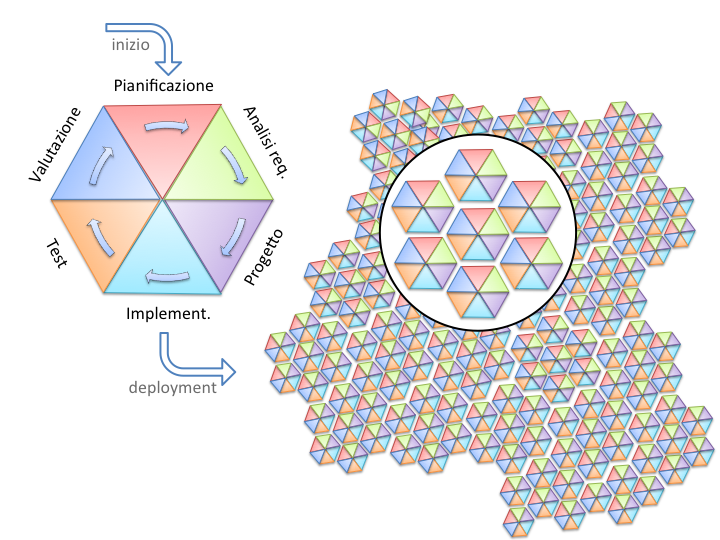
\includegraphics[scale=0.5]{img/modello_incrementale.png}
		\caption{Rappresentazione del modello incrementale\protect\footnotemark}
		\label{fig:modello_incrementale}
	\end{figure}

	\footnotetext{Fonte in \S\ref{rifinfo}}
	
    \section{Processi Primari}\label{PP}

    \subsection{Processo di fornitura}\label{PP:Fornitura}	%istanziare Management Process, Infrastructure Process e Improvement Process

        \subsubsection{Scopo}\label{PP:Fornitura:Scopo}
		La sezione corrente ha lo scopo di riportare le  attività principali del fornitore in rapporto con il cliente. 
		
		\subsubsection{Ricerca delle tecnologie}
		Il gruppo approfondisce la propria conoscenza su tecnologie e framework vari, in modo da discutere insieme quali sono quelle di interesse comune e di utilità per il progetto. Questo prevede poi l'auto-formazione di quelle scelte in comune accordo per averne una buona padronanza.

        \subsubsection{Studio di Fattibilità}\label{PP:Fornitura:SdF} 
        In quest'attività viene prodotto il documento \DAlt{\textit{Studio di Fattibilità v1.0}} al fine di analizzare ogni capitolato e scegliere quale contratto accettare. 
        Nello specifico, il documento in ogni sezione contiene:
        	\begin{itemize}
        		\item \textbf{Descrizione generale}: breve descrizione del capitolato.
        		\item \textbf{Obiettivo finale}: punto focale su cui si concentra.
        		\item \textbf{Tecnologie coinvolte}: elenco delle tecnologie direttamente coinvolte esplicitate nel capitolato.
        		\item \textbf{Valutazione conclusiva}: giudizio finale del gruppo.
        	\end{itemize}
        
        \subsubsection{Preparazione in vista della revisione}
        In questa parte il gruppo prepara tutto il materiale necessario al buon superamento della revisione, come per esempio lettera di presentazione, documentazione e slide per l'esposizione.


    \subsection{Processo di sviluppo}\label{PP:Sviluppo}

        \subsubsection{Scopo}\label{PP:Sviluppo:Scopo}
        Cont


        \subsubsection{Analisi dei Requisiti}\label{PP:Sviluppo:AdR}
        Contenuto generico
        
        

		 \paragraph{Denominazione dei requisiti}\label{PP:Sviluppo:AdR:DenominazioneRequisiti}
		 Scrivere codice univoco per requisiti
		 Priorità - Tipo (se funzionale ecc) - Codice (?)
	
		 \paragraph{Casi d'uso}\label{PP:Sviluppo:AdR:CasiUso}
		 %descrivere cos'è?
		 La denominazione scelta per i casi d'uso è la seguente
		 \begin{itemize}
		 	\item UC[NUMERO] per uno principale (ad esempio, per il primo caso d'uso UC1)
		 	\item UC[NUMERO].[NUMERO] per un sotto caso (ad esempio, per il primo sotto caso del primo caso d'uso UC1.1)	
		 \end{itemize}
	 	 %ecc..
		        
	        %\subparagraph{Gerarchie di casi d'uso}\label{PP:Sviluppo:AdR:CasiDUso:GerarchieCasiDUso}	% SOLO SE UTILE
	        %Contenuto


        %\subsubsection{Progettazione}\label{PP:Sviluppo:Progettazione}	%PIÙ AVANTI
        %Contenuto generico
        

		 %\paragraph{Obiettivi}\label{PP:Sviluppo:Progettazione:Obiettivi}
		 %Contenuto



		\subsubsection{Diagrammi UML}\label{PP:Sviluppo:UML}	
		
		
        %\paragraph{Codifica}\label{PP:Sviluppo:Codifica} %PIÙ AVANTI

        
        \subsubsection{Strumenti}\label{PP:Sviluppo:Strumenti}
        
	    \paragraph{Ambiente di sviluppo}\label{PP:Sviluppo:Strumenti:AmbienteSviluppo}
	    Vengono qui riportate le componenti software utilizzate da ogni membro del gruppo per lo sviluppo del progetto.
	         	
	        	
	    \subparagraph{Sistema operativo}\label{PP:Sviluppo:Strumenti:AmbienteSviluppo:SistemaOperativo}
	    
	    Ubuntu 18.
	        		
	    %\subparagraph{IDE}\label{PP:Sviluppo:Strumenti:AmbienteSviluppo:IDE}
	    %Atom - Intellij?
        
		
		
	
    \section{Processi Organizzativi}


    \subsection{Gestione del progetto}

	    \subsubsection{Scopo}
	    Questa sezione ha lo scopo di delineare in cosa consiste l'attività di gestione del progetto.

	    % \subsubsection{Istanziazione dei processi}	%da rivedere
		% Derivano dagli standard...

		\subsubsection{Pianificazione delle attività}

			\paragraph{Scopo delle pianificazione}
			Si occupa di generare il PdP e comprende:
			\begin{itemize}
				\item Risorse
				\item Assegnazione delle risorse alle attività
				\item ...
				..
			\end{itemize}

			\paragraph{Obiettivi}
			L'attività è importante per...
			Struttura generale del PdP:
			\begin{itemize}
				\item Introduzione e scopo;
				\item Analisi;
				\item Modello di sviluppo adottato..
				..
			\end{itemize}

			\paragraph{Procedura}
			Procedura generale per l’organizzazione della pianificazione.
			con politiche di gestione dei rischi..

			\paragraph{Ruoli di progetto}
			I ruoli\footnote{Per la descrizione completa, vedere ``Descrizione dei ruoli di progetto'' in \S\ref{rifinfo}.} scelti per lo sviluppo del progetto sono:
			\begin{itemize}[noitemsep]
				\item Analista
				\item Progettista
				\item Responsabile
				\item Amministratore
				\item Programmatore
				\item Verificatore
			\end{itemize}


		\subsubsection{Pianificazione della qualità}
		In tale sezione vengono descritte le metriche e l'utilizzo di strumenti utili ad ottenere qualità nei processi, nei documenti e nei prodotti. Alcuni di questi strumenti sono già stati descritti \Doc{\PdQ} che i vari standard adottati. Gli obiettivi che ci si pone di raggiungere con questi strumenti sono anch'essi descritti nel \Doc{\PdQ}.
		
			\paragraph{Standard usati per perseguire la qualità}		
			Gli standard presi come riferimento a cui si può dare un risultato quantitativo sono:
			
			\begin{itemize}
				\item \textbf{ISO/IEC 15504}
				\item \textbf{Ciclo di Deming}
			\end{itemize}
		
				\subparagraph*{ISO/IEC 15504}
				Ogni processo attivato verrà classificato e valutato secondo gli attributi assegnati ai vari livelli di qualità.
				
				Per ogni attributo verrà infine indicata una percentuale di quanto il processo rispetti l'attributo, potendo infine capire nel complesso quanto quel processo riesca a superare un dato livello di maturità.
				
				\subparagraph*{Ciclo di Deming}
				Nel fase migliorativa del processo sarà data particolare attenzione nel non iniziale una fase del ciclo di Deming senza aver finito completamente le fasi precedenti.
			
			\paragraph{Classificazione degli obiettivi}
			Gli obiettivi per la qualità (Q) concordati dall'\Amm~e dal \Ver~ descritti nel \PdQ~avranno il seguente codice identificativo:
			
			\begin{center}
				Q[Tipo][ID]: Nome
			\end{center}
		
			\begin{itemize}
				\item \textbf{Tipo}: indica il la tipologia dell'oggetto di cui viene valutata la qualità, e questa può essere:
				\begin{itemize}
					\item \textbf{PR}: processi;
					\item \textbf{PD}: prodotti che risultano essere documenti;
					\item \textbf{PS}: prodotti software;
				\end{itemize}
			
				\item \textbf{ID}: ogni tipo di obiettivo possiede una lista ordinata attraverso un numero incrementale di tre cifre;
				\item \textbf{Nome}: offre un'informazione più chiara dell'obiettivo attraverso una breve frase;
			\end{itemize}
		
			Ad esempio:
			
			\begin{itemize}
				\item \textbf{QPD001: Leggibilità del testo}
			\end{itemize}
			
			
			\paragraph{Classificazione delle metriche}
			Ogni obiettivo della qualità deve per quanto possibile essere collegato ad una metrica, anch'essa scelta dall'\Amm~e dal \Ver. Questo per valutare quantitativamente il raggiungimento o meno degli obiettivi stabiliti.
			
			Le metriche (M) verranno classificate nel seguente modo:
			
			\begin{center}
				M[Tipo][ID]: Nome
			\end{center}
			
			\begin{itemize}
				\item \textbf{Tipo}: indica il la tipologia dell'oggetto di cui viene applicata la metrica, e questa può essere:
				\begin{itemize}
					\item \textbf{PR}: processi;
					\item \textbf{PD}: prodotti che risultano essere documenti;
					\item \textbf{PS}: prodotti software;
				\end{itemize}
				
				\item \textbf{ID}: ogni tipo di obiettivo possiede una lista ordinata attraverso un numero incrementale di tre cifre;
				\item \textbf{Nome}: offre un'informazione più chiara dell'obiettivo attraverso una breve frase;
			\end{itemize}
		
			Ad esempio:
			
			\begin{itemize}
				\item \textbf{MPD001: Indice Gulpease}
			\end{itemize}
		
			Quando sarà possibile, la metrica e l'obiettivo di qualità collegati fra loro avranno lo stesso Tipo e ID.
			
			Ad esempio:
		
			\begin{table}[H]
				\begin{detailtable}{\columnwidth}{YYYY}
					\thead{ID} & 
					\thead{Nome} &
					\thead{Descrizione} &
					\thead{Metrica}\\\hline\rowcolor{gray!15}
					QPD001 &Leggibilità del documento &La lettura del documento deve essere comprensibile &MPD001: Gulpease				\end{detailtable}
			\end{table}
			
		\subsubsection{Controllo del progetto}

			\paragraph{Monitoraggio del progetto}

			\subparagraph{Monitoraggio dell'esecuzione dei processi}
			Ogni processo verrà controllato periodicamente durante tutta la sua esecuzione in modo da non intralciare il way of working,
			mediante misurazioni associate a metriche descritte dai processi di verifica, controllate tramite l'utilizzo di strumenti automatizzati.
			Le metriche adottate sono, per il processo considerato, indicatori di efficacia dei prodotti rispetto ai requisiti di funzionalità e qualità,
			stabiliti nel \Doc{\PdQ\ v1.0.0} e nell'\Doc{\AdR v1.0.0}. Risultano validi indicatori per la valutazione di:
			\begin{itemize}
				\item Aderenza al way of working
				\item Stato di avanzamento del processo rispetto alla pianificazione
				\item Identificazione dei problemi
				\item Eventuali ripianificazioni
			\end{itemize}

			\subparagraph{Procedure di comunicazione}
			Per coordinare il team e il committente sullo stato del progetto sono state stabilite le seguenti norme:
			\begin{itemize}
				\item Per le comunicazioni interne verranno utilizzati gli strumenti segnalati in \S\ref{pianificazione e coordinamento}, in particolare
					con l'utilizzo di \gloss{Slack} e, all'occorrenza, verranno fissate riunioni per le questioni più importanti:
					\begin{itemize}
						\item concordare data, ora e luogo;
						\item stabilire un ordine del giorno da discutere;
						\item appuntare il contenuto della riunione per poter poi redigere formalmente il verbale della riunione
					\end{itemize}
				\item Per le comuncazioni esterne verrà utilizzata prevalentemente la comunicazione via email. % HELP WANTED fissare riunioni con l'azienda?
			\end{itemize}


    		\paragraph{Gestione dei problemi emersi}
			Problemi emersi durante l'esecuzione dei processi verranno segnalati tramite ticket, utilizzando il sistema integrato di Github come descritto
			in dettaglio in \S\ref{Github}. Questo permette di tracciare i problemi insorti durante le attività e di pianificare la risoluzione degli stessi.

    		% \paragraph{Riportare lo stato di avanzamento del progetto}
			% vedere Breaking Bug, io non riesco a capire il senso di questo paragrafo e lo toglierei ~ Tim

		\subsubsection{Chiusura dei processi}

    		\paragraph{Archiviazione dei prodotti}
			I prodotti che, una volta terminate le attività e processi per completarli, soddisfano le aspettative in termini di qualità,
			verranno archiviati in apposite \gloss{repository}. Alla versione attuale di questo documento, RIVEDERE

    		\paragraph{Archiviazione delle misurazioni} % TODO
    		necessario archiviare le misurazioni effettuate attraverso le metriche definite nel presente documento..

    	\subsubsection{Strumenti di pianificazione e coordinamento}\label{pianificazione e coordinamento}

    		\paragraph{Slack} %da Telegram, trasferirsi
			Slack è uno strumento di collaborazione sviluppato appositamente per coordinare il lavoro tra i team, permettendo la comunicazione in tempo
			reale, e mettendo a disposizione molte altre utilità indispensabili. Tra queste, c'è la possibilità di dividere il \gloss{workspace} in vari canali
			specifici, marcare parole o frasi importanti con diversi stili (grassetto, corsivo, codice, barrato), fissare i messaggi importanti, aprire un \gloss{thread}
			sotto ogni messaggio per non creare \gloss{spam} sul canale, ecc \dots

			Il workspace usato dal team è stato suddiviso in diversi canali, in base alle esigenze del periodo di lavoro. Nel periodo attuale, i vari canali sono:
			\begin{itemize}
				\item \textbf{\# general}: canale in cui verranno discusse tematiche generali riguardanti il progetto e le sue attività.
				\item \textbf{\# Analisi dei Requisiti}: discussioni inerenti alla stesura del documento \Doc{\AdR}. Nello specifico verranno discussi
					 i requisiti e i casi d'uso.
				\item \textbf{\# Piano di Progetto}: discussioni inerenti la pianificazione, la suddivisione del lavoro, la valutazione dei rischi, la consuntivazione e
					altre attività volte alla redazione del documento \Doc{\PdP}.
				\item \textbf{\# Piano di Qualifica}: discussioni inerenti principalmente la qualità di processo e di prodotto, riportate nel documento \Doc{\PdQ}.
				\item \textbf{\# Norme di Progetto}: discussioni riguardanti le norme che il gruppo adotterà e che ogni membro sarà tenuto a rispettare. Esse
					saranno riportate nel documento \Doc{\NdP}.
				\item \textbf{\# Studio di Fattibilità}: canale in cui verrà discussa la fattibilità di ogni capitolato proposto, convergenti nel documento
					\Doc{\SdF}.
				\item \textbf{\# git}: canale in cui un bot correttamente configurato manderà una notifica ogni volta che verrà effettuato un commit, oppure alla chiusura o apertura
					di una issue nel repository principale.
				\item \textbf{\# latex}: discussioni riguardanti gli aspetti tecnici di \LaTeX.
				\item \textbf{\# random}: discussioni \gloss{off-topic} del team.
			\end{itemize}

    		\paragraph{GitHub}\label{Github}
			Github fornisce un servizio di tracking delle issue per ogni repository che ospita. Questo strumento offre più funzionalità di quanto potrebbe
			sembrare, poichè permette anche di trattare le issue come delle \gloss{task}, marcandole con una opportuna label. Infatti, l'issue tracker offre le seguenti
			funzionalità:
			\begin{itemize}
				\item Aprire una issue, attribuendone un titolo e una descrizione più dettagliata. Ogni issue è legata a un ID che verrà automaticamente generato (e.g. \texttt{\#32}),
					al quale sarà possibile fare riferimento nei messaggi di commit.
				\item Creare delle \gloss{milestone}, e aggregare ad esse le issue.
				\item Assegnare delle label alle issue, per marcarne la natura. Ad esempio, una issue marcata come bug sarà un problema da risolvere,
					una issue marcata come enhancement sarà un miglioramento o una task. È possibile inoltre creare delle label personalizzate.
				\item Assegnare un issue a un collaboratore, che sarà tenuto a correggerla.
				\item Supporto di \gloss{markdown} esteso, che permette di formare delle pagine per le issue di aspetto delizioso e allo stesso tempo estremamente funzionali.
			\end{itemize}

			%\paragraph{Redmine} % ? da vedere piu avanti.
			% Per ora Github per issue-task tracker ~Tim



	\subsection{Formazione}

		La formazione di ogni membro del gruppo avviene tramite studio autonomo dei \gloss{framework} menzionati da \II\ durante la presentazione del progetto e incontri con AlphaSix.

		\subsubsection{Piano di formazione}
		Il piano di formazione prevede:
		\begin{itemize}
			\item Lo studio della documentazione di tecnologie e metodologie quali:
			\begin{itemize}
				\item Redmine
				\item GitLab
				\item SonarQube
				\item Apache Kafka
				\item Telegram
				\item Slack
				\item Docker
				\item API Rest
				\item The Twelve-Factor App %!! TODO aggiungere in Studio di fat
			\end{itemize}
			\item Lo studio delle possibilità d'integrazione tra di esse
		\end{itemize}


    
\section{Processi di supporto}\label{PS}

	\subsection{Documentazione}\label{PS:Documentazione}

		\subsubsection{Implementazione}\label{PS:Documentazione:Implementazione}

			\paragraph{Template}\label{PS:Documentazione:Implementazione:Template}
			Prima di iniziare a redigere i documenti, è stato creato un \gloss{template} per \LaTeX \ (\S\ref{LaTeX}) contenente tutte le impostazioni grafiche condivise tra questi, per sfruttare il riutilizzo del codice e semplificare enormemente la manutenzione dei sorgenti.\par
			Nello specifico, è presente un file per ognuna delle seguenti utilità:
			\begin{itemize}
				\item \gloss{Layout} delle pagine
				\item \gloss{Macro} personalizzate volte a semplificare l'utilizzo di strutture o comandi ricorrenti
				\item Codice per la generazione della prima pagina
					(struttura definita in \S\ref{PS:Documentazione:Struttura:Frontespizio})
				\item Diario delle modifiche
			\end{itemize}

			\paragraph{Ciclo di vita dei documenti}\label{PS:Documentazione:Implementazione:CicloVita}
			Durante il suo ciclo di vita, ogni documento potrà trovarsi in una delle seguenti fasi:
			\begin{itemize}
				\item \textbf{Redazione}: fase che inizia con la creazione del documento e dura fino alla sua ultima approvazione.
					Il \Res\ assegna ai \gloss{redattori} le varie sezioni di ogni documento da redigere, i quali aggiorneranno la versione nel diario delle modifiche
					come normato in \S\ref{Versionamento}.
				\item \textbf{Verifica}: il documento entra in questa fase nel momento in cui i Redattori hanno terminato la stesura del lavoro loro assegnato, segnalandolo al \Res, che a sua volta assegnerà ai Verificatori la verifica della qualità del prodotto, secondo quanto riportato nelle norme di verifica. Essi potranno approvare il documento oppure notificare il \Res\ su eventuali errori o incongruenze emerse durante la fase di verifica, che provvederà a riassegnare il lavoro.
				\item \textbf{Approvazione}: fase che inizia dall'accettazione del documento da parte dei Verificatori nella fase di verifica. Spetta al \Res\
					l'approvazione ufficiale del documento, seguita dal rilascio di una \gloss{major release}.
			\end{itemize}

		\subsubsection{Struttura}\label{PS:Documentazione:Struttura}

			\paragraph{Frontespizio}\label{PS:Documentazione:Struttura:Frontespizio}
			La prima pagina di ogni documento, eccezione fatta per i verbali (in cui saranno presenti informazioni ridotte), sarà caratterizzata da:
			\begin{itemize}
				\item Logo e nome del gruppo
				\item Titolo del documento
				\item Informazioni sul documento:
					\begin{itemize}
						\item Versione documento
						\item Data di creazione e ultima modifica
						\item Nominativo dei Redattori
						\item Nominativo dei Verificatori
						\item Nominativo del \Res
						\item Destinazione d'uso
						\item Destinatari del documento
						\item Contatto del gruppo
					\end{itemize}
				\item Breve descrizione del documento
			\end{itemize}

			\paragraph{Storico delle versioni}\label{PS:Documentazione:Struttura:StoricoVersioni}
			La pagina che segue il frontespizio contiene lo storico delle versioni del documento, in cui ogni aggiunta o modifica significativa ha
			comportato un incremento di versione. Ogni riga contiene, a partire da sinistra:
			\begin{itemize}
				\item Il numero della versione nel formato espresso in \S\ref{Versionamento}
				\item Una breve descrizione delle modifiche apportate
				\item Il ruolo dell'autore che ha apportato la modifica
				\item Il nominativo dell'autore
				\item La data di modifica
			\end{itemize}
			La chiave primaria della tabella è il numero di versione ordinata in senso decrescente, in modo che la versione più vecchia sia
			l'ultima riga della tabella.

			\paragraph{Indice}\label{PS:Documentazione:Struttura:Indice}
			In ogni documento, esclusi i verbali, è presente un indice contenente tutte le sezioni, sottosezioni e paragrafi. I numeri di sezioni, sottosezioni,
			e paragrafi sottostanti saranno separati da un punto (e.g. 1.4.1).\par
			Saranno eventualmente presenti un indice delle
			figure e un indice delle tabelle, assenti in caso non ci siano tabelle o figure nel documento.\par
			I valori degli indici partono da 1.

			\paragraph{Contenuto}\label{PS:Documentazione:Struttura:Contenuto}
			La struttura di ogni pagina presenta:
			\begin{itemize}
				\item Intestazione con:
				\begin{itemize}
					\item A sinistra, logo di \emph{\gruppo}
					\item A destra, nome del capitolato e documento corrente
				\end{itemize}
				\item Piè di pagina con:
				\begin{itemize}
					\item A sinistra, nome e mail di riferimento del gruppo
					\item A destra, numero della pagina corrente
				\end{itemize}
			\end{itemize}


		\subsubsection{Design}\label{PS:Documentazione:Design}

			\paragraph{Norme tipografiche}\label{PS:Documentazione:Design:NormeT}
			Le norme tipografiche qui di seguito elencate sono state decise in modo che ogni membro di \gruppo\ concorra a mantenere una forma coerente e univoca
			per tutti i documenti redatti.

			\subparagraph{Stile del testo}\label{PS:Documentazione:Design:NormeT:StileTesto}
			\begin{itemize}
				\item \textbf{Corsivo}: solo per i nomi dei documenti citati.
				\item \textbf{Maiuscolo}: la prima lettera per
				\begin{itemize}
					\item tutte le parole appartenenti ai nomi dei documenti tranne gli articoli
					\item i nomi dei ruoli
				\end{itemize}
			\end{itemize}

			\subparagraph{Elenchi puntati}\label{PS:Documentazione:Design:NormeT:ElenchiPuntati}
			\begin{itemize}
				\item \textbf{Simboli di livello}: un pallino nero per il primo livello, un trattino per il secondo livello.
				\item \textbf{Punteggiatura}: nessuna punteggiatura alla fine di una frase, tranne nel caso in cui sia presente una descrizione.
					In quel caso la descrizione è preceduta dai due punti ``:'' e termina con un punto ``.''.
				\item \textbf{Grassetto}: solo se è presente una descrizione, allora sono in grassetto tutte le parole prima dei due punti ``:''.
			\end{itemize}

			\subparagraph{Altri formati testuali comuni} \label{PS:Documentazione:Design:NormeT:AltriFormati}
			\begin{itemize}
				\item \textbf{Orari}: \texttt{HH:MM} secondo la norma ISO 8601 nel formato 24 ore dove:
				\begin{itemize}
					\item \texttt{HH} indica le ore, da 00 a 23
					\item \texttt{MM} i minuti, da 00 a 59
				\end{itemize}
				\item \textbf{Date}: \texttt{DD-MM-YYYY} formato adottato in Europa dove:
				\begin{itemize}
					\item \texttt{DD} indica il numero del giorno, da 01 a 31
					\item \texttt{MM} il mese, da 01 a 12
					\item \texttt{YYYY} l'anno
				\end{itemize}
				\item \textbf{Nota a piè di pagina}: serve ad inserire elementi aggiuntivi, come osservazioni o riferimenti a parti interne al documento, utili alla comprensione del testo, ma se inseriti all'interno del discorso ne interromperebbero la lettura rendendola meno scorrevole.
			\end{itemize}


			\paragraph{Elementi grafici}

			\subparagraph{Figure}
			Ogni immagine inserita nei documenti deve sempre essere centrata rispetto al foglio e adeguatamente separata dal testo. Deve inoltre essere
			accompagnata da una breve \gloss{caption} che permetta al lettore di capire esattamente che cosa sta guardando.\\
			È presente nell'indice l'elenco delle figure che raccoglie la lista di tutte le immagini presenti.

			\subparagraph{Tabelle}
			Come per le figure, ogni tabella sarà accompagnata da una caption e sarà della dimensione del testo, o se più piccola, centrata.
			Tutte le tabelle saranno raccolte nell'elenco delle tabelle.\par
			Saranno presenti due tipologie di tabelle:
			\begin{itemize}
				\item \textbf{Semplici}: tabelle standard senza uno stile particolare, in cui le celle sono separate da bordi neri (evitare, ove non risulta necessario,
					le righe verticali).
				\item \textbf{Complesse}: tabelle con un'alternanza di colori tra le righe delle celle (grigio e bianco) e senza bordi verticali.
					Le celle sono separate orizzontalmente da una corretta spaziatura e allineamento e verticalmente dall'alternanza dei due colori.
					La riga dell'\gloss{header} può essere bianca o di un grigio più scuro in base al contesto, con il testo che può essere in grassetto.
			\end{itemize}


		\subsubsection{Produzione}

			\paragraph{Suddivisione dei documenti}

			\subparagraph{Documenti interni}
			Sono considerati interni documenti quali \SdF\ e \NdP\ che non sono visibili ad entità esterne, ma solo ad \gruppo.

			\subparagraph{Documenti esterni}
			Sono considerati esterni, invece, documenti quali \PdP, \PdQ\ e \AdR\ che, al contrario dei precedenti, sono visibili al committente.
			
			%Questi documenti sono ufficiali e approvati direttamente dal \Res\ e comprendono, per esempio: \PdP, \PdQ\ e \AdR. Si chiamano esterni perché accessibili al committente.

			%\subparagraph{Glossario} 
			% TODO: già scritto nell'introduzione, eliminare? L: anche sì
			%Il documento denominato \Doc{\Gl}  raccoglie in ordine alfabetico tutti i termini utilizzati che necessitano di una spiegazione più approfondita.
			%Sono identificabili all'interno degli altri documenti da un font differente e una G a pedice la prima volta che appaiono.


			\subparagraph{Verbali}
			Questi documenti vengono successivamente alle riunioni tenute da \gruppo\ o in caso di incontri con \gloss{stakeholder} esterni, per esempio con \II. Vengono redatti da una singola persona e presentano tutti le stesse sezioni:
			%Questi documenti vengono redatti quando \gruppo\ tiene delle riunioni o ci sono incontri esterni, per esempio con \II. Vengono redatti da una singola persona e presentano tutti le stesse sezioni:
			\begin{itemize}
				\item \textbf{Informazioni incontro}: lista delle informazioni principali riguardanti la riunione quali luogo, data, orario, ordine del giorno, ecc\dots
				\item \textbf{Argomenti}: lista dei principali argomenti trattati con descrizione di cosa si è discusso nel dettaglio.
				%TODO: da riempire se viene aggiunto altro
			\end{itemize}


			\paragraph{Strumenti di supporto}

			\subparagraph{\LaTeX} \label{LaTeX}
			Per la stesura della documentazione è stato scelto di usare il linguaggio di \gloss{markup} \LaTeX \ perché presenta molti vantaggi, tra i quali:
			\begin{itemize}
				\item Supporta nativamente il versionamento, essendo un linguaggio compilato
				\item Supporta la modularità, rendendo più facile organizzare un documento dividendone logicamente i vari moduli
				\item Permette il riutilizzo del codice tramite l'uso di macro già pronte o personalizzate, oppure includendo lo stesso sorgente in punti diversi
					(ad esempio come fatto in \S\ref{PS:Documentazione:Implementazione:Template})
				\item Gestisce automaticamente indici e riferimenti
			\end{itemize}

			\subparagraph{TexStudio/Visual Studio Code}
			TexStudio e Visual Studio Code sono i due ambienti di sviluppo scelti da \gruppo\ per stilare la documentazione.
			TexStudio è un \gloss{IDE} nativo per l'utilizzo di \LaTeX. Visual Studio Code è un editor intelligente moderno (alla pari di un \gloss{IDE}) che, tramite
			estensioni, permette il supporto di praticamente ogni linguaggio.
			Entrambi permettono una rapida compilazione e un'istantanea visualizzazione dell'anteprima del PDF prodotto, oltre agli altri vantaggi che ogni IDE offre,
			tra cui: suggerimenti e completamenti automatici delle parole chiave, ricerca intelligente (eventualmente tramite \gloss{regexp}) controllo ortografico della
			lingua italiana o inglese e così via.\\
			Più informazioni sono reperibili sui rispettivi siti ufficiali, i cui link sono presenti in \S\ref{rifinfo}.
			% \subparagraph{Visual Studio Code}

			\subparagraph{GanttProject} % TODO: Rivedere?
			GanttProject è un programma gratuito dedicato alla formazione dei diagrammi di Gantt. Permette di creare task e milestone, organizzare le task in lavoro strutturato a interruzioni, disegnare i vincoli di dipendenza tra di esse e molte altre utilità, generando automaticamente il relativo diagramma.
			Per maggiori informazioni, si rimanda alla fonte ufficiale (consultare \S\ref{rifinfo}).

			\subparagraph{Draw.io}
			Draw.io è un'applicazione web in grado di creare diagrammi UML, di Entità-Relazionale, di flusso e molto altro. Il motivo che ha portato AlphaSix a scegliere questo strumento è la sua perfetta integrazione con \gloss{Google Drive}, oltre al suo alto livello di intuitività. Questo vantaggio permette poter condividere i diagrammi creati tra tutti i collaboratori in ogni momento e in modo automatico. Per maggiori informazioni, visualizzare la fonte ufficiale (\S\ref{rifinfo}).

			\subparagraph{Indice di Gulpease}
			Per il calcolo dell'indice di Gulpease, è stato creato uno script ad hoc che, preso in input un file PDF, produce in output l'indice Gulpease.
			È stato scelto come accettabile un indice con valore compreso tra 50 e 60 per i documenti che seguiranno le norme qui definite.

		\subsubsection{Mantenimento}

			\paragraph{Versionamento} \label{Versionamento}
			Tutti i documenti redatti supportano il versionamento, in modo da essere univoci e per rendere disponibile la possibilità di consultare versioni precedenti in qualsiasi fase del loro \gloss{ciclo di vita}.
			Il modello di versionamento adottato segue lo schema \gloss{change significance}.\\La versione di un file è espressa secondo la notazione
			\begin{center}
				\texttt{vX.Y.Z}
			\end{center}
			\indent dove:
			\begin{itemize}
				\item \texttt{X} indica il numero di versione principale. Inizia da 0 e viene incrementato ogni volta che il \Res\ approva il documento, determinando	una major release.
				\item \texttt{Y} indica il numero di versione secondario, contatore delle fasi di verifica effettuate dal \Ver\ superate positivamente. Inizia da 0. 	Viene azzerato ad ogni incremento della \texttt{X}.
				\item \texttt{Z} è l'indice di modifica minore, incrementato ogni volta che viene effettuato un aggiornamento inferiore, quale l'aggiunta di una sezione	o correzioni grammaticali/sintattiche di un certo peso. Viene azzerato ad ogni incremento della \texttt{Y} o della \texttt{X}.
			\end{itemize}

			%\texttt{X}, \texttt{Y} e \texttt{Z} hanno dominio $[0,+\infty)$, possono assumere pertanto un valore $> 9$.

			\paragraph{Continuous Integration}
			Per quanto riguarda la stesura dei documenti, verrà adottato il principio di \gloss{Continuous Integration}, che sarà tuttavia limitato in questo periodo
			a sincronizzarsi il prima possibile con il repository remoto (non essendoci
			una vera e propria build o dei test da effettuare), sia per quanto riguarda il \gloss{fetch} che per il \gloss{push}.

			Questo serve a rendere più remota possibile la probabilità di incappare nell'\gloss{Integration Hell}.


			\paragraph{Nomenclatura}

			\subparagraph{Verbali}	\label{NomenclaturaVerbali}
			I Verbali  possono essere interni oppure esterni, nel caso in cui il team incontri gli esponenti di \II.
			Il nominativo del file in cui sono formalizzati è il seguente:
			\begin{itemize}
				\item \texttt{VI\_dd-mm-yyyy.pdf} per i verbali interni
				\item \texttt{VE\_dd-mm-yyyy.pdf} per i verbali esterni
			\end{itemize}
			dove dd-mm-yyyy è la data in cui sono stati tenuti, nel formato descritto nel paragrafo \S\ref{PS:Documentazione:Design:NormeT:AltriFormati}.

			\subparagraph{Documenti vari}
			Saranno presenti due tipologie di file: file interni ad \gruppo\ e file esterni.
			\begin{itemize}
				\item La prima categoria include moduli di \LaTeX\ contenenti le varie sezioni e che non verranno mai esposti esternamente. Questi file verranno	denominati usando la convenzione \texttt{snake\_case.tex}, dove snake\_case è il nome della sezione o modulo.
				\item La seconda categoria include i file \texttt{.tex} principali che produrranno i PDF da consegnare al committente. Essi verranno denominati con la convenzione \texttt{CamelCase\_vX.Y.Z.pdf}, dove CamelCase sarà il nome del documento generico mentre	\texttt{vX.Y.Z} sarà la versione che identifica univocamente il documento come descritto in \S\ref{Versionamento}.
			\end{itemize}

	\subsection{Verifica}

		\subsubsection{Scopo}
		Questa sezione vuole descrivere come il team di sviluppo esegue la fase di verifica, per capire se i prodotti e i processi sono conformi a quanto ci si attende.
		La fase di verifica serve per stabilire se è opportuno o meno procedere alla fase successiva del progetto, se ciò non fosse possibile sarà necessario il
		ritorno ad una fase stabile del progetto per poi ripartire da lì prendendo in considerazione i risultati della precedente verifica.

		%\subsubsection{Aspettative} %da mettere nel PdQ

		\subsubsection{Descrizione}
		Ogni processo e prodotto deve essere valutato in modo quantificabile attraverso metriche apposite, quando possibile, e stabilendo il risultato che si vuole raggiungere.

		Come indicato dal \textit{Ciclo di Deming} nel \Doc{\PdQv} all'appendice \S A, nel momento in cui tale risultato sarà raggiunto, se esso non è il migliore,
		servirà come ``base'' per alzare il livello di qualità di quel processo o prodotto.

		I risultati ottenuti nella fase di verifica sono riportati nel \PdQ, in questo modo, confrontandoli con gli esiti attesi,
		è possibile valutare un miglioramento per i vari processi e prodotti sempre nel \PdQ.
		
		\subsection{Walkthrough e Inspection}
		Due modi di effettuare la verifica sono attraverso Walkthrough e Inspection. Il team di sviluppo li adotta entrambi, ma non contemporaneamente, per i vantaggi che comporta ogni metodo.
		
			\subsubsection*{Walkthtough}
			Metodo di verifica che effettua un controllo ad ampio spettro senza l’assunzione di presupposti. Dato che per mettere in atto tale metodo ci si deve divide in gruppi dove ognuno ha un ruolo ben distinto, Walkthrough è ideale per le verifiche effettuate all'inizio dei vari periodi, dove i membri del team di sviluppo non possiedono le conoscenze adeguate per una verifica efficiente.
			
			Walkthrough possiede delle fasi ben specifiche:
			
			\begin{enumerate}
				\item \textbf{Pianificazione}: viene pianificato in gruppo come effettuare la verifica dei prodotti.
				\item \textbf{Lettura}: viene effettuata la lettura del prodotto.
				\item \textbf{Discussione}: vengono discusse le possibili correzioni.
				\item \textbf{Correzione di difetti}: si attuano i risultati ottenuti dalla fase di discussione.
			\end{enumerate}
		
		\subsubsection*{Inspection}
		Metodo di verifica dove si esegue una lettura mirata dei prodotti, frutto di un'analisi dei risultati sei precedenti test. Questo metodo dunque, a differenza di Walkthrough, prevede l'esecuzione con dei presupposti.
		
		Le fasi di Inspection sono:
		
		\begin{enumerate}
			\item \textbf{Pianificazione}: viene sempre pianificato in gruppo come effettuare la pianificazione.
			\item \textbf{Definizione di una lista di controllo}: dato che le parti da verificare sono specificate, queste possono essere riportate in una lista in modo da velocizzare il processo di verifica.
			\item \textbf{Correzione dei difetti}: attuazione dei punti della lista di controllo.
		\end{enumerate}
	
	Per la natura di Inspection, questa non può essere applicata fin dall'inizio, dunque nel momento in cui si presentano nuove tipologie di prodotti e processi da verificare viene effettuato Walkthrough, nel momento in cui il metodo di verifica è ben consolidato da tutti i membri del team di sviluppo si passa ad effettuare verifica secondo Inspection.  
		
		\subsubsection{Metriche}
		La denominazione delle metriche è già stata descritta in \S\ref{Classificazione metriche}, qui viene descritto il loro funzionamento.
			\paragraph{Metriche per i documenti}
				\subparagraph{MPD001 Indice Gulpease}
				Si tratta di un indice di leggibilità dei documenti in lingua italiana. A differenza degli indici per le altre lingue, questo si basa sulla
				lunghezza delle parole in lettere e non in sillabe. L'indice si calcola:

				\[89+\dfrac{300\times n_{\text{frasi}}-10\times n_{\text{lettere}}}{n_{\text{parole}}}\]

				\textbf{Metrica}: il risultato della formula è interpretato nel seguente modo

				\begin{itemize}
					\item \textbf{<80}: documento  difficile da leggere per chi ha la licenza elementare;
					\item \textbf{<60}: documento  difficile da leggere per chi ha la licenza media;
					\item \textbf{<40}: documento difficile da leggere per chi ha un diploma superiore;
				\end{itemize}

				Nel momento in cui avviene un commit all'interno di repository, in automatico si avvia uno script che analizza tutti i documenti in PDF per valutarne l'indice Gulpease. I risultati vengono poi riportati in un apposito file di testo per verificarne la qualità ed un possibile miglioramento.

%				\subparagraph{MPD002 Correttezza ortografica}
%				Gli errori ortografici possono essere segnalati dallo strumento di Controllo Ortografico presente in \textit{TexStudio}.
%
%				\textbf{Metrica}: il numero di errori ortografici presenti nel documento.

			\paragraph{Metriche per i processi}
				\subparagraph{MPR001 Varianza della pianificazione}
				Nella sezione \S 1.5 del documento \Doc{\PdPv} sono stabilite le \gloss{baseline} e le scadenze di consegna dei vari prodotti.
				Nonostante il tempo di slack che ogni fase possiede, è possibile che delle date non vengano rispettate causa incidenti di vario tipo che sono
				analizzati nella sezione \S 2 del \Doc{\PdPv}, intitolata Analisi dei rischi.

				\[\dfrac{\sum_{i=1}^{n} x_i}{n}\]
				
				$x_i=\text{numero di giorni di ritardo per la i-esima scadenza.}$

				\textbf{Metrica}: viene indicata la media di giorni di ritardo nel rispettare una scadenza durante il macro periodo. Se un'attività viene conclusa con in d'anticipo, il numero di giorni di ritardo non è negativo ma nullo.
				
				\subparagraph{MPR002 Varianza dei costi}
				All'interno della sezione \S 6 del \Doc{\PdPv} è indicato il costo approssimativo del progetto.
				In corso d'opera possono presentarsi dei problemi che richiedono un'aggiunta di costo in termini di $\frac{\text{tempo}}{\text{persona}}$.
				Lo scopo del preventivo è infatti quello di fare una stima non definitiva dei costi. Per verificare se il preventivo è rispettato viene fatto periodicamente un consuntivo di periodo.

				\textbf{Metrica}: viene misurata la differenza conteggiata in \euro\ tra il costo finale e il preventivo.
				Viene seguito tale schema per la tariffa oraria dei vari ruoli del team di sviluppo:

				\begin{itemize} % TODO: tabellina?
					\item \textbf{Responsabile}: \euro\ 30
					\item \textbf{Amministratore}: \euro\ 20
					\item \textbf{Analista}: \euro\ 25
					\item \textbf{Progettista}: \euro\ 22
					\item \textbf{Programmatore}: \euro\ 15
					\item \textbf{Verificatore}: \euro\ 15
				\end{itemize}

				\subparagraph{MPR003 Aderenza agli standard}
				Per misurare e verificare i processi sono stati scelti alcuni specifici standard di qualità descritti nel \PdQ che possono offrire una valutazione quantitativa.
				Gli standard scelti sono:

				\begin{itemize}
				\item \textbf{ISO/IEC 15504}: ogni processo attivato verrà classificato e valutato secondo gli attributi assegnati ai vari livelli di qualità. Per ogni attributo verrà infine indicata una percentuale di quanto il processo rispetti l'attributo, potendo infine capire nel complesso quanto quel processo riesca a superare un dato livello di maturità;
				\item \textbf{Ciclo di Deming}: nella fase migliorativa del processo sarà data particolare attenzione nel non iniziare una fase del \textit{Ciclo di Deming} senza aver finito completamente le fasi precedenti;
				\end{itemize}

				\textbf{Metrica}: il livello di maturità descritto nell'ISO/IEC 15504 all'appendice §A del \Doc{\PdQv}.

				\subparagraph{MPR004 Frequenza commit nella repository}
				Per mantenere aggiornate le versioni dei prodotti è necessario che ogni membro di \gruppo\ effettui un commit ad ogni sua modifica significativa.
				Così facendo, in caso di errori, è possibile tornare ad una versione stabile del progetto.				
				Misurare quanti commit sono stati effettuati inoltre serve per monitorare l'attività del team di sviluppo.
				\[\dfrac{\sum_{i=1}^{n} x_i}{n}\]
				$x_i=\text{numero di commit alla i-esima settimana del macro periodo.}$\\
				\textbf{Metrica}: numero minimo di commit da effettuare in media ogni settimana lavorativa durante un macro periodo.

				\subparagraph*{Metriche sui requisiti e i rischi}
				Dato che non è fisso il numero dei requisiti di un progetto, sono state scelte una serie di metriche dove il valore ottimale da raggiungere è sempre uguale,
				lo zero. È stato scelto di contare il numero di requisiti non soddisfatti invece che il contrario. Lo stesso ragionamento è valido per quanto
				riguarda i rischi che possono verificarsi nel corso del progetto.

				Gli obiettivi che si vogliono raggiungere attraverso tali metriche possono essere stabiliti solo a progetto concluso.

				\subparagraph{MPR005 Requisiti obbligatori non soddisfatti}
				Per adempiere completamente alla richiesta del cliente, serve individuare tutti i requisiti presenti nella sua richiesta, impliciti, espliciti, diretti e derivati. Alcuni sono imprescindibili, detti obbligatori, e il loro soddisfacimento determina la buona riuscita del progetto.

				\textbf{Metrica}: numero dei requisiti obbligatori non soddisfatti.

				\subparagraph{MPR006 Requisiti desiderabili non soddisfatti}
				I requisiti desiderabili non sono necessari, ma offrono un valore aggiunto al progetto.

				\textbf{Metrica}: numero dei requisiti desiderabili non soddisfatti.

				\subparagraph{MPR007 Requisiti opzionali non soddisfatti}
				Tali requisiti dovranno essere adempiuti solo nel momento in cui tutti i requisiti obbligatori saranno soddisfatti.
				Possono essere concordati col cliente in corso d'opera.

				\textbf{Metrica}: numero dei requisiti opzionali non soddisfatti.

				\subparagraph{MPR008 Rischi non previsti avvenuti} % TODO: Rivedere l'ultima frase
				Nell'Analisi dei rischi presente nella sezione §2 del \Doc{\PdPv}, sono presenti i rischi ritenuti possibili per i quali è proposta una soluzione.
				Possono presentarsi anche rischi non previsti in tale analisi. Questi devono essere il meno possibili (nulli) perché la loro soluzione sarà decisa al momento causando ritardi all'interno del progetto.

				\textbf{Metrica}: numero di rischi non previsti avvenuti nel corso dell'intero progetto.

				\paragraph{MPR009 Frequenza controllo prodotti}
				I documenti e i prodotti software hanno bisogno di una verifica frequente, commisurata in base al numero di modifiche che vengono apportate.

				Chi esegue la modifica deve controllare ciò che ha fatto prima di poter ufficializzare, mentre la verifica fatta dal \Ver\ deve essere fatta solo nel momento in cui è stato raggiunto un numero significativo di modifiche, per evitare di spendere troppe risorse in questa fase.
			
				\[\dfrac{\sum_{i=1}^{n} x_i}{n}\]
				$x_i=\text{numero di modifiche effettuate prima della i-esima verifica.}$
				\textbf{Metrica}: media del numero massimo di modifiche apportate ai prodotti prima che ricevano una verifica dal parte del \Ver.

			\paragraph{Analisi statica}
			L'analisi statica verifica solo i prodotti che non sono o che non possono essere eseguiti, come i documenti.

				\subparagraph{Analisi dei documenti}
				L'analisi statica per i documenti si limita a valutare come e con che contenuti questi vengono scritti.
				Per l'analisi dei documenti vengono utilizzate:

				\begin{itemize}
					\item \textbf{MPD001}
					\item \textbf{MPD002}
				\end{itemize}

%TODO: non facciamo ora analisi dinamica!
%			\paragraph{Analisi dinamica}
%			L'analisi dinamica valuta il comportamento dei prodotti in esecuzione, verificando se restituiscono i risultati attesi e se operano nel modo stabilito.
%			Vengono presi in esame i prodotti software e i processi.

				\subparagraph{Analisi dei processi}
				Per analizzare i processi vengono usati gli standard sopra elencati. Ad ogni fase del processo verranno valutati gli attributi richiesti secondo l'ISO 15504 e in che misura questi sono stati rispettati e in che fase del \textit{Ciclo di Deming} il processo si trova.
				Per l'analisi dei processi vengono utilizzate:

				\begin{itemize}
					\item \textbf{MPR001 Varianza della pianificazione}
					\item \textbf{MPR002 Varianza dei costi}
					\item \textbf{MPR004 Frequenza commit nella repository}
					\item \textbf{MPR009 Frequenza controllo prodotti}
					% \item \textbf{MPR010 Norme di progetto non seguite}
				\end{itemize}


				%\paragraph{...Tutti i test}	%UTILE??

				%\paragraph{Strumenti}

				%\subparagraph{Verifica di documentazione}
				%Google Docs?

				%\subparagraph{Integrazione continua} % Jenkins? Più avanti?


\end{document}
